\documentclass[../skript.tex]{subfiles}
	\section{A summary of point mechanics}\label{c1se2}

		A particle occupies a finite volume. However, often it's practical to describe it as a single \underline{point} particle, located at the center of mass. This works also for big objects, as e.g. planets.
		\subsection*{Our physical system}
			In a physical syste mwe have $N$ point particles with masses $m_i>0,\,i=1,...,N$. These particles are moving in $\mathbb{R}^d$ (typically $d=3$).
			\begin{itemize}
				\item [a)] \textbf{Kinematics }movement\par 
					$\vec x_i(t)\in\mathbb{R}^d,\,i=1,...,N$ and $t>0$ is the position of the $i$-th particle at time $t$. Analogeously $\vec v_i(t) = \vec x_i'(t)$ is the velocity of the $i$-th particle at time $t$. If \underline{no} force acts on the particles $\Rightarrow$ Trajectory of the $i$-th particle is a line:
					\begin{IEEEeqnarray*}{rCl}
						\vec v_i(t) &=& \vec v_i(0),\quad \forall t\forall i\\
						\vec x_i(t) &=& \vec x_i(0) + t\vec v_i(0),\quad\forall t\forall i.
					\end{IEEEeqnarray*}
				\item [b)] Forces modify the trajectory. We have two types of forces acting on particle $i$:
					\begin{enumerate}
						\item External forces $\vec f_i(t)$
						\item Internal forces among the particles: $f_{i,j}(t)$ is the force applied on $i$ due to interaction with the $j$-th particle
					\end{enumerate} 
				The effect of the forces on the trajectory is described by Newton's 2nd law:
				\[
					\text{force} = \text{mass}\cdot\text{acceleration}.
				\]
				Thus for particle $i$ it holds that
				\begin{equation}\label{*}\tag{*}
					m_i\vec x_i''(t) = \underbrace{F_i}_{\text{total force acting on }i} = \vec f_i + \sum_{j=1,j\neq i}^N \vec f_{i,j}
				\end{equation}
				\cref{*} is called the \textbf{equation of motion for the $i$-th particle}.

			\subsection*{Constraints on the form of $\vec f_{i,j}$}
				We have a mutual interaction between two particles, so the force does not just act in one direction (from one particle to another). Newton's 3rd law states that
				\[
					\text{force on $i$ due to $j$} = -\text{force acting on $j$ due to $i$}
				\]
				so
				\[
					\vec f_{i,j}(t) = - \vec f_{j,i}(t)
				\]
				$\Rightarrow$ $\vec f_{i,j}$ \underline{must be} of the form 
				\[
					\vec f_{i,j} = \frac{\vec x_i-\vec x_j}{|x_i-x_j|}\cdot g_{i,j}(|x_i-x_j|)
				\]
				for a scalar function $g_{i,j}$ with $g_{i,j} = g_{j,i}$.\par 
				In $d=3$ we have some examples:
				\begin{itemize}
					\item \textbf{Gravitational force:}\[
						g_{i,j}(\tau) = - \frac{G m_im_j}{\tau^2}
					\]
					where $m_i>0$ is the mass and $G$ is the gravity constant
					\item \textbf{Electrical force:} 
					\[
						g_{i,j}(\tau) = K\frac{Q_iQ_j}{\tau^2}
					\]
					where $Q_i$ is the charge of the particle $j$
				\end{itemize}
				Here we $|\vec x|$ to denote the euclidean norm for some $\vec x\in\mathbb{R}^d$.\par 
				Till now we just considered the interaction between $2$ particles of the system. There are more constraints to be considered, which appear if we consider the whole system of $N$ particles $\Rightarrow$ \textbf{Conservation laws}

				\item [c)]\textbf{Conservation laws}
					\begin{itemize}
						\item [$c_1)$] \textbf{Conservation of momentum:}
						\[
							m_i\vec v_i = m_i\vec x_i' = \vec p_i
						\]
						is called the \textbf{momentum of the particle $i$}. The \textbf{equation of momentum for the $i$-th particle} can be written as
						\[
							\vec p_i'=  F_i
						\]
						which is the total force acting on $i$. \par 
						Let 
						\begin{IEEEeqnarray*}{rCl}
							\vec p(t) &=& \sum_{i=1}^N \vec p_i(t) = \text{total momentum}\\
							\vec f(t) &=& \sum_{i=1}^N \vec f_i(t) = \text{total external force}.
						\end{IEEEeqnarray*}
						Then
						\begin{equation}\label{eq_c1}\tag{c1}
							\vec p'(t) = \vec f(t)
						\end{equation}
						Note that in the equation of momentum for one particle we have external \underline{and} internal forces, whereas in \cref{eq_c1} just external forces appear!
						\begin{proof}[Proof of \cref{eq_c1}]
							We have
							\begin{IEEEeqnarray*}{rCl}
								\vec p'(t) &=& \sum_{i=1}^N p_i'(t)\\ &=& \sum_{i=1}^N F_i(t)\\
								&=& \underbrace{\sum_{i=1}^N\vec f_i(t)}_{\eqqcolon f} + \underbrace{\sum_{i=1}^N\sum_{j=1,j\neq i}^N f_{i,j}}_{=\frac{1}{2}\sum_{i\neq j}\underbrace{(f_{i,j}+f_{j,i})}_{=0}}.
							\end{IEEEeqnarray*}
						\hspace{1mm}\end{proof}
						\item [$c_2)$]
						\begin{figure}[ht]
							\centering
							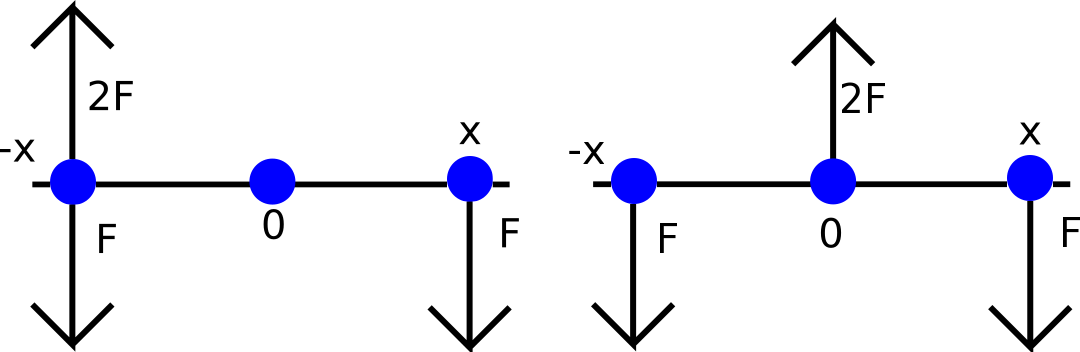
\includegraphics[width=0.4\textwidth]{Images/pde4.png}
							\caption{Two examples of force diagrams}
							\label{fig4}
						\end{figure}
						 \textbf{Conservation of angular momentum:}\newline\noindent In both cases of \cref{fig4} we have total force equal to zero, but in the example on the left we have (clockwise) rotation.
					\end{itemize}
			\end{itemize}
			\begin{definition}\label{def1.1}
				For $d=3$ the \textbf{cross product} (vector product) is defined as
				\begin{eqnarray*}
					x:&\mathbb{R}^3\times\mathbb{R}^3&\to\mathbb{R}^3\\
					&(a,b) &\mapsto \vec a\times \vec b = |a|\,|b|\sin \Theta
				\end{eqnarray*}
				where $\Theta\in[0,\pi)$ is the angle between $a$ and $b$. $\vec n$ is the unit vector $\perp$ to the plane spanned by $a$ and $b$ and its direction is given by the `right hand rule':
				\begin{IEEEeqnarray*}{rCl}
					(a\times b)_1 &=& a_2b_3-a_3b_2\\
					(a\times b)_2 &=& a_3b_1-a_1b_3\\
					(a\times b)_3 &=& a_1b_2-a_2b_1.
				\end{IEEEeqnarray*}
				It has the properties $a\times b = - b\times a$ and $a\times a = 0$.\par
				We can represent the cross product by the \emph{Levi-Civita} symbol $\varepsilon^{i,j,k}$: \newline\noindent
				Let $\pi(1,2,3) = \pi(1)\pi(2)\pi(3)$ and 
				\[
					\varepsilon^{\pi(1)\pi(2)\pi(3)} = \signe{\pi}
				\]
				with $\varepsilon^{123} = 1 = \varepsilon^{312} = \varepsilon^{231}$. We have
				\[
					\varepsilon:(1,2,3)^3 \to \{0,1,-1\} \text{ with } (i,j,k)\mapsto \varepsilon^{ijk}.
				\]
				It holds that $\varepsilon^{ijk} = 0$ if two f the indices coincide, otherwise we have $\varepsilon^{ijk} = \signe \pi$. Then
				\[
					(a\times b)_i = \sum_{j,k=1}^3 \varepsilon^{ijk}a_jb_k.
				\]
			\end{definition}
			\begin{definition}\label{def1.2}
				The \textbf{angular momentum of the \underline{external force} on the $i$-th particle} (the \underline{torque}) is defined as
				\[
					\vec M_i \coloneqq (\vec x_i-\vec x_0)\times\vec f_i,
				\]
				where $\vec x_0$ is a \underline{fixed} reference point in $\mathbb{R}^3$.
			\end{definition}
			\begin{definition}\label{def1.3}
				The \textbf{angular momentum of the $i$-th particle} is defined as
				\[
					\vec L_i \coloneqq (\vec x_i-\vec x_0)\times \vec p_i.
				\]
			\end{definition}
			\begin{itemize}
			\item 
				\begin{itemize}
					\item [$c_2$] \textbf{Conservation of angular momentum:} \par 
					Let 
					\begin{eqnarray*}
						\vec L &=& \sum_{j=1}^N \vec L_j\\
						\vec M &=& \sum_{j=1}^N \vec M_i
					\end{eqnarray*}
					be the \textbf{total angular momentum}, resp. the \textbf{total torque}. Then
					\begin{equation}\label{eqn_c2}\tag{c2}
						\vec L'(t) = \vec M(t).
					\end{equation}
					\begin{proof}
						We have
						\begin{IEEEeqnarray*}{rCl}
							L'&=&\sum_{i=1}^N  L_i'\\
							&=& \sum_{i=1}^N \left( (x_i-x_0)\times p_i \right)' \\
							&=& \sum_{i=1}^N \underbrace{x_i'\times p_i}_{m_i x_i'\times x_i'= 0} + \sum_{i=1}^N (x_i-x_0)\times p_i'\\
							&=& \sum_{i=1}^N (x_i-x_0)\times\underbrace{p_i'}_{\text{equal mot.}}\\
							&=& \sum_{i=1}^N (x_i-x_0) \times \underbrace{F_i}_{=\underbrace{f_i}_{\text{external}}+\underbrace{\sum_{j=1,j\neq i}^N f_{i,j}}_{\text{internal}}}\\
							&=& \underbrace{\sum_{i=1}^N (x_i-x_0)\times f_i}_{=M} + \underbrace{\sum_{i=1}^N\sum_{j=1,j\neq i}^N (x_i-x_0)\times f_{i,j}}_{\coloneqq A}
						\end{IEEEeqnarray*}
						where
						\begin{IEEEeqnarray*}{rCl}
							A&=& \frac{1}{2}\sum_{i=1,i\neq j}^N (x_i-x_0)\times f_{i,j} + (x_j-x_0)\underbrace{f_{j,i}}_{=-f_{i,j}}
						\end{IEEEeqnarray*}
						and from $A$ terms cancel out using Newton's 3rd Law.
					\hspace{1mm}\end{proof}
					\begin{example}
						\begin{figure}
							\centering
							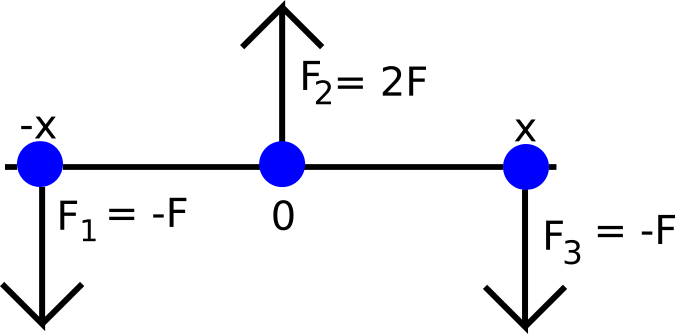
\includegraphics[width=0.4\textwidth]{Images/pde5.png}
							\caption{A force diagram}
							\label{fig5}
						\end{figure}
						As seen in \cref{fig5} the total force is $F_1 + F_2 + F_3 = 0 \Rightarrow P'= 0$. Using $x_0 = 0$ the total torque is 
						\begin{equation*}\left.
						\begin{aligned}
							\vec M_1 &=& (x_1-x_0)\times F_1 = \vec x\times\vec F\\
							\vec M_2 &=& (x_2-x_0)\times F_2 = -\vec x\times \vec F = - M_1\\
							\vec M_3 &=& \underbrace{(x_0-x_0)}_{=0}\times F_3 = 0
						\end{aligned}\right\}
						\Rightarrow M_1 + M_2 + M_3 = 0 \Rightarrow L'= 0
						\end{equation*}
						thus the system is \underline{not rotating!}
					\end{example}
					Another example:
					\begin{example}
						\begin{figure}[ht]
							\centering
							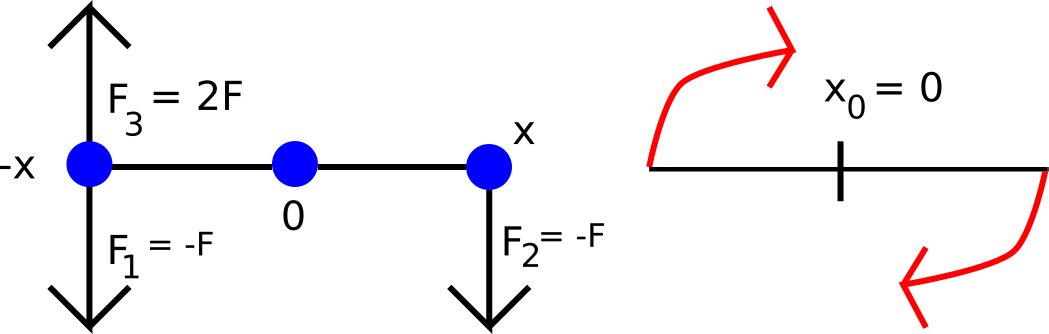
\includegraphics[width=0.4\textwidth]{Images/pde6.png}
							\caption{A force diagram and the resulting rotation of the system}
							\label{fig6}
						\end{figure}
						For the situation in \cref{fig6} we have that the total force $\tilde F_1 + F_2 =0$ and $P'= 0$, so there is no translation. However, the total torque is
						\begin{equation*}
							\left.
								\begin{aligned}
									M_1 &=& (x_1-x_0)\times\tilde F_1 = -\vec x\times\vec F\\
									M_2 &=& (x_2-x_0)\times F+2 = -\vec x\times\vec F
								\end{aligned}
							\right\}
							\Rightarrow M_1+M_2 = -2\vec x\times\vec F \neq 0\Rightarrow \underbrace{L'\neq 0}_{\text{System rotates!}}
						\end{equation*}
					\end{example}

					\item [$c_3)$] Energy conservation:\par 
					The energy of a particle system consists of kinetic energy (form movement) and internal energy (potential energy) from interactions between the particles. The kinetic energy (energy `stored' in the movement) is given by
					\[
						E_k = \sum_{i=1}^N \frac{|x_i'(t)|^2}{2}m_i = \sum_{i=1}^N \frac{|P_i|^2}{2m_i}.
					\]
					For the potential energy, $E_p$, we need an 
					\begin{assumption}
						$E_p$ can be influenced \underline{only} by internal forces!
					\end{assumption}
					To quentify we need the definition of `work':
					\begin{definition}
						We define the \textbf{work} done per unit time on the particle $i$ by the force $F_i$ by
						\[
							w_i \coloneqq \vec F_i\cdot\vec x_i',\quad [w] = \text{force}\cdot\frac{\text{displacement}}{\text{time}}.
						\]
					\end{definition}
					In our case we have
					\[
						w_i = \underbrace{f_i\cdot x_i'}_{w_i^{\eqqcolon\text{ext}}} + \underbrace{\sum_{j=1,j\neq i}^N f_{i,j}\cdot x_i'}_{\eqqcolon w_i^{\text{int}}}.
					\]
					$E_p$ is controlled by internal forces only, i.e.
					\[
						E_p'(t) = -w_{\text{int}}(t)
					\]
					where
					\[
						w_{\text{int}} \coloneqq \sum_{i=1}^N w_i^{\text{int}}
					\]
					\underline{Claim: } $E_k'= w_{ext} + w_{int}$ with $w_{ext} = \sum_{j=1}^N w_j^{ext}$ and $w_{int} = \sum_{j=1}^N w_j^{int}$.
					\begin{proof}
						We know 
						\begin{IEEEeqnarray*}{rCl}
							E_k' &=& \frac{d}{dt} \left( \sum_{i=1}^N \frac{m_i}{2} x_i'\cdot x_i' \right)\\
							&=& \sum_{i=1}^N \underbrace{m_i x_i''}_{=F_i = f_i + \sum_{j=1,j\neq i}^N f_{i,j}}\cdot x_i'\\
							&=& \underbrace{\sum_{i=1}^N f_i\cdot x_i'}_{=w_{ext}}+ \underbrace{\sum_{i=1}^N\sum_{j=1,j\neq i}^N f_{i,j}\cdot x_i'}_{= w_{int}}
						\end{IEEEeqnarray*}
						\hfill
					\hspace{1mm}\end{proof}
					The claim and the assumption together give us the \textbf{conservation of total energy}: Let $E(t) = E_k + E_p$. Then
					\begin{equation}\label{eqn_c3}\tag{c3}
						E'= w_{ext}.
					\end{equation}
					\textbf{Form of the potential}\newline\newline\noindent
					\underline{Claim:} Assume $E_p'= -w_{int}$. Then 
					\[
						E_p(t) = -\frac{1}{2}\sum_{j=1,j\neq i}^N G_{i,j}(|x_i-x_j|),
					\]
					where if 
					\[
						\vec f_{i,j} = \frac{\vec{x_i-x_j}}{|x_i-x_j|} g_{i,j}(|x_i-x_j|)
					\]
					then $G(\tau)$ is a primitive(?) of $g(\tau)$ (with $g_{i,j} = g_{j,i}$).
					\begin{proof}
						\begin{IEEEeqnarray*}{rCl}
							E_p'&=& -w_{int} \\
							&=& - \sum_{i=1}^N (\sum_{j=1,j\neq i}^N x_i'\cdot f_{i,j})\\
							&=& -\frac{1}{2}\sum_{i\neq j} (\vec x_i'\cdot \vec f_{i,j} + \vec x_j'\cdot\vec f_{j,i})\\
							&=& -\frac{1}{2} \sum_{i\neq j} \vec f_{i,j}\cdot(x_i'-x_j')\\
							&=& -\frac{1}{2} \sum_{i\neq j} \frac{(\vec{x_i-x_j})}{|x_i-x_j|}\cdot(\vec x_i-\vec x_j)' \cdot \underbrace{g_{i,j}(|x_i-x_j|)}_{=G_{i,j}'(|x_i-x_j|)}\\
							&=& -\frac{1}{2} \sum_{i\neq j} \frac{d}{dt} G_{i,j} (|x_i(t)-x_j(t)|)
						\end{IEEEeqnarray*}
					\hspace{1mm}\end{proof}
				\end{itemize}
			\end{itemize}